\documentclass[sigconf,review,anonymous]{acmart}

\usepackage{booktabs} % For formal tables

% Copyright
\setcopyright{none}
%\setcopyright{acmcopyright}
%\setcopyright{acmlicensed}
%\setcopyright{rightsretained}
%\setcopyright{usgov}
%\setcopyright{usgovmixed}
%\setcopyright{cagov}
%\setcopyright{cagovmixed}


% DOI
\acmDOI{10.475/123_4}

% ISBN
\acmISBN{123-4567-24-567/17/06}

%Conference
\acmConference[SIGGRAPH 2017 Posters]{SIGGRAPH 2017 Posters}{August 2017}{Los Angeles, CA, USA} 
\acmYear{2017}
\copyrightyear{2017}
\acmPrice{15.00}

% use the "authoryear" citation style.
\citestyle{acmauthoryear}
\setcitestyle{square}

\begin{document}
\title{GRNsight: a web application and service for visualizing models of small- to medium-scale gene regulatory networks}

\author{Eileen Choe}
\orcid{1234-5678-9012}
\affiliation{%
  \institution{Loyola Marymount University}
  \streetaddress{1 LMU Drive}
  \city{Los Angeles} 
  \state{California} 
  \postcode{43017-6221}
}
\email{trovato@corporation.com}

\author{G.K.M. Tobin}
\affiliation{%
  \institution{Institute for Clarity in Documentation}
  \streetaddress{P.O. Box 1212}
  \city{Dublin} 
  \state{Ohio} 
  \postcode{43017-6221}
}
\email{webmaster@marysville-ohio.com}

% The default list of authors is too long for headers}
\renewcommand{\shortauthors}{B. Trovato et. al.}

\begin{abstract}

GRNsight is a web application and service optimized for visualizing small- to medium-scale gene regulatory networks (GRNs). A GRN consists of genes, transcription factors, and the regulatory connections between them which govern the level of expression of mRNA and protein from genes. GRNsight produces weighted or unweighted network graphs from an Excel spreadsheet containing an adjacency matrix where regulators are named in the columns and target genes in the rows, a Simple Interaction Format (SIF) text file, or a GraphML XML file. GRNsight represents genes as nodes and regulatory connections as edges with colors, end markers, and thicknesses corresponding to the sign and magnitude of activation or repression. GRNsight visualizations can be modified through manually dragging nodes or adjusting sliders that change the force graph parameters. GRNsight is best-suited for visualizing networks of fewer than 35 nodes and 70 edges, and has general applicability for displaying any small, unweighted or weighted network with directed edges for systems biology or other application domains. The GRNsight application (http://dondi.github.io/GRNsight/) and code (https://github.com/dondi/GRNsight) are available under the open source BSD license.

\end{abstract}

%
% The code below should be generated by the tool at
% http://dl.acm.org/ccs.cfm
% Please copy and paste the code instead of the example below. 
%
\begin{CCSXML}
<ccs2012>
<concept>
<concept_id>10003120.10003145.10003147.10010364</concept_id>
<concept_desc>Human-centered computing~Scientific visualization</concept_desc>
<concept_significance>500</concept_significance>
</concept>
<concept>
<concept_id>10003120.10003145.10003151.10011771</concept_id>
<concept_desc>Human-centered computing~Visualization toolkits</concept_desc>
<concept_significance>500</concept_significance>
</concept>
</ccs2012>
\end{CCSXML}

\ccsdesc[500]{Human-centered computing~Scientific visualization}
\ccsdesc[500]{Human-centered computing~Visualization toolkits}

% We no longer use \terms command
%\terms{Theory}

\keywords{Scientific Visualization, Software Engineering, Bioinformatics}

\begin{teaserfigure}
  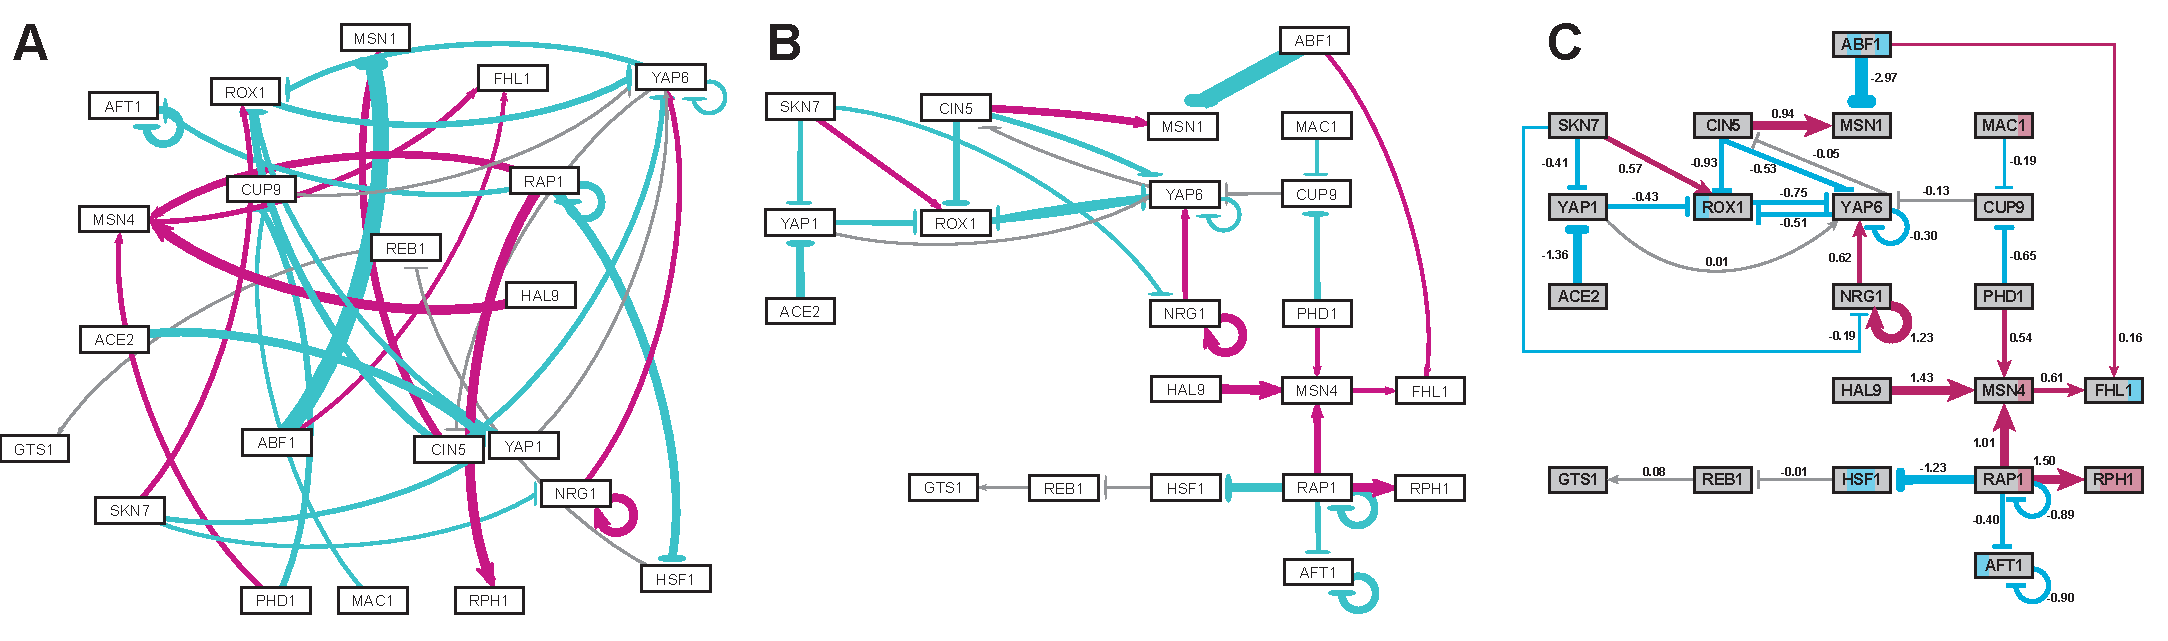
\includegraphics[width=\textwidth]{comparison.pdf}
  \caption{Side-by-side comparison of the same adjacency matrices laid out by GRNsight and by hand. (A) GRNsight automatic layout of the demonstration file, Demo #4: Weighted GRN (21 genes, 31 edges); (B) graph from (A) manually manipulated from within GRNsight; (C) the same adjacency matrix from (A) and (B) laid out entirely by hand in Adobe Illustrator.}
  \label{fig:teaser}
\end{teaserfigure}


\maketitle

\section{Introduction and Motivation}

GRNsight is a web application and service for visualizing models of small- to medium-scale gene regulatory networks (GRNs). A gene regulatory network (GRN) consists of genes, transcription factors, and the regulatory connections between them which govern the level of expression of mRNA and protein from genes. The original motivation came from our efforts to perform parameter estimation and forward simulation of the dynamics of a differential equations model of a small GRN with 21 nodes and 31 edges, and quickly and easily visualize the weight parameters from the model. A review by Pavlopoulos et al. \cite{doi:10.1186/s13742-015-0077-2}, describes the types, trends, and usage of 47 visualization tools available for genomics and systems biology available at our project inception in January 2014. However, our use case was narrow, because we wanted a tool for novice and experienced biologists alike to quickly and easily view unweighted and weighted network graphs, and the tools we investigated out of this diverse set each had properties that limited their use for us. Thus, we enumerated the following requirements for a potential visualization tool. The tool should:

\begin{enumerate}
\item Exist as a web application without the need to download and install specialized software;
\item Be simple and intuitive to use;
\item Automatically lay out and display small- to medium-scale, unweighted and weighted, directed network graphs in a way that is familiar to biologists and adds value to the interpretation of the modeling results.
\end{enumerate}

\section{Materials and Methods}

\subsection{Input Data}
\begin{figure}[ht]
  \centering
  \includegraphics[width=3.0in]{Figure1_zoom100.png}
  \caption{Screenshot of the expected format for an adjacency matrix for an unweighted network.}
  \label{fig:Screenshot}
\end{figure}

GRNsight can automatically lay out either an unweighted or weighted network graph specified by an adjacency matrix where regulators are named in the columns and target genes in the rows in a worksheet named 'network' or 'network\_optimized\_weights' in a Microsoft Excel workbook (.xlsx). Note that regulators (regulatory transcription factors) are themselves encoded by genes and will be referred to as such.

\subsection{Graph Customizations and User Interface}
\begin{figure}[ht]
  \centering
  \includegraphics[width=3.0in]{screenshot.png}
  \caption{Screenshot of GRNsight user interface.}
  \label{fig:Screenshot}
\end{figure}
GRNsight's diagrams are based on force graph layout algorithms in the D3.js visualization library \cite{d3}, which was then extensively customized to support the specific needs of biologists for GRN visualization. The GRNsight user interface includes a menu/status bar and sliders that adjust D3.js's force graph layout parameters. Users can move force graph parameter sliders to refine the automated visualization. Nodes have a charge, which repels or attracts other nodes. The charge distance determines at what range a node's charge will affect other nodes. The link distance determines the minimum distance maintained between nodes. Gravity determines the strength of the force drawing the nodes to the center of the graph. Sliders can be locked to prevent changes and also reset to default values. Graph visualizations can also be modified through manual node dragging. Design decisions for the user interface were driven by applicable interaction design guidelines and principles \cite{norman2013design,shneiderman2010designing,nielsen1994usability} in alignment with the mental model and expectations of the target user base, consisting primarily of biologists.

\subsection{Data Interoperability}


\section{Results and Discussion}
We have successfully implemented GRNsight, a web application and service for visualizing small- to medium-scale GRNs, fulfilling our 3 requirements.

(summary of the comparison and the conclusions reached from the GRNsight visualization)

Thus, GRNsight enables one to interpret the weight parameters more easily than one could from the adjacency matrix alone. Visual inspection has long been recognized by experts such as Tufte (2001) and Card, Mackinlay & Shneiderman (1999) as distinct from other forms of purely numeric, computational, or algorithmic data analysis, and as the preceding discussion highlights, it is this potential that can be derived specifically by visual inspection that is enabled by GRNsight. Tufte's (2001) seminal book perhaps states it best: 'Graphics reveal data. Indeed graphics can be more precise and revealing than conventional statistical computations.'

\subsection{Improvements and Feature Additions in GRNsight v2}


\section{Conclusion and Future Work}
We have successfully implemented GRNsight, a web application and service for visualizing small- to medium-scale GRNs that is simple and intuitive to use. GRNsight accepts an input file, reading reading a weighted or unweighted representation of a GRN, and automatically lays out and displays unweighted and weighted network graphs in a way that is familiar to biologists. It has general applicability for displaying any small, unweighted or weighted network with directed edges for systems biology or other application domains. Thus, GRNsight inhabits a niche not satisfied by other software, doing 'one thing well.'
~future work here...~

\bibliographystyle{ACM-Reference-Format}
\bibliography{siggraph-abstract-review} 

\end{document}
